\section{Authentication}
\begin{parag}{What is authentication?}
	\begin{definition}{(Authentication)}
    The process of verifying a claimed identity
    \end{definition}
	
\end{parag}
\begin{framedremark}
	Be careful: authentication must not to be confused with \important{message authentication} in which we verifying 
	\begin{itemize}
	    \item Message provenance
	    \item Message integrity
	\end{itemize}
\end{framedremark}

\begin{parag}{Where does Authentication fit?}
	The question that we need to answer first before thinking of the how is the where, where should authentication fit? From what we have seen in the past week (weeks 2 and 3), we know that between the path from a request to the completion by the TCB  have authorization, access control. Recall that \important{access control} establishes whether a principal is authorized to operate on an asset. Before the access control mechanism can make this decision, \important{authentication} needs to happen to ensure that the principal is who he says he is.
	\begin{subparag}{Remark}
	    We will mostly cover authentication of \important{users}, and a bit of machine authentication.
	\end{subparag}
\end{parag}


\begin{parag}{Where to prove who you are}
    There is a lot of way to prove who we are, there are traditionals one with 
	\begin{itemize}
	    \item \textbf{What you know} password, secret key
	    \item \textbf{What you are} biometrics
	    \item \textbf{What you have} Smart card, secure token
	\end{itemize}
	And some more modern 
	\begin{itemize}
	    \item \textbf{Where you are} location, IP address
	    \item \textbf{How you act} behavioural authentication
	    \item \textbf{Who you know} social ties
	\end{itemize}
	And many others ...
\end{parag}

\begin{parag}{What you know: Passwords}
	\begin{definition}{(Password)}
    Secret shared between user and system
    \end{definition}
	It works by the user having a secret password and the system checking it to authenticate the user. However this gives us a lot of problems to solve 
	\begin{itemize}
	    \item \textbf{Secure transfer}: the password may be eavesdropped when communicated
	    \item \textbf{Secure check}: naive checks may leak information about the password
	    \item \textbf{Secure storage}: if stolen the full system is compromised
	    \item \textbf{Secure passwords}: easy-to-remember passwords tends to be easy to guess
	\end{itemize}
	The secrecy of the password depends on how easy it is to predict. If the password can be guessed, it does not matter all the above is secured. The password is still not secret.
\end{parag}

\begin{parag}{Secure transfer}
    Well as seen before, if we were to sent the password in clear through the communication channel, anyone with an access to it could impersonate the user. Hence as we have already seen in the class, what we require here is to have a secure transfer: encrypt the tuple $\left(\text{login}, \text{password}\right)$ in transit so that it cannot be eavesdropped. Typically one does not just encrypt this information, one also \important{encrypt the channel} using a standard protocol (e.g. TLR, HTTPS which combines the concepts we have seen in a safe way). As always do \textbf{NOT} build your own protocol.
\end{parag}


\begin{parag}{Beware of replay attacks}
    Well, encrypting the password may not be enough here right? Imagine if an eavesdropper just copied the encrypted message that Alice has sent to Bob and resend, Bob wouldn't have any way to see whether or not it was Alice or Eve. Even if the password is encrypted, one can copy the content and then reply the encrypted content.
\end{parag}
\begin{parag}{Challenge-Response protocols}
    To avoid reply attacks (for passwords and in general) one usually uses \important{Challenge-Response} protocols. In these protocols:
	\begin{enumerate}
	    \item The principal that wants to authenticate first declares their intention to login
	    \item The party authenticating the principal sends a \important{challenge}, a random number (from a large space, to ensure that there are no repetitions and cannot be predicted)
	    \item The principal encrypts the password together with the challenge. This ensures that 
			\begin{enumerate}
			    \item The password is never encrypted to the same value
			    \item the encryption is fresh (i.e., corresponds to the declaration in step 1)
			\end{enumerate}
	\end{enumerate}
	After checking the password, the authenticating party \important{must} delete the challenge so that the message cannot be replied.\\
	$ $\\
	When Bob receives the tuple, in order to be sure that this tuple indeed authenticates Alice, Bob needs to know what is the correspondence between Alice and her password. This is typically stored in some sort of database. And as always, if the password are stored in the clear, an adversary can read them (e.g., in UNIX the password file is readable by anyone!) and then use them to impersonate the users. Also, remember the asymmetry of the adversary vs. the defender. We do not need all adversaries to be able to read the passwords or breach into the database. It suffices that one attacker gets access and leaks the passwords of millions of people (fortunately most of these database are not in the clear, although that does not mean they are safe). A first idea can be to encrypt the passwords under storage. When Bob receives the password, decrypts it, and check the challenge. If the challenge is fresh, then to check if it corresponds to the encryption stored in the database he can 
	\begin{enumerate}
	    \item Encrypt the received password and compare it to the stored value
	    \item Decrypt the stored password and compare it to the encrypted value
	\end{enumerate}
	But note that the encryption is as secure as the security of the key. To encrypt/decrypt the passwords the key needs to be on the same machine, so if the adversary can access the database, he can also steal the key. Hence we need a primitive that does not require a key and allows for checking, a \important{hash function}. When Bob receives the password, he decrypts it, and checks the challenge. If the challenge is fresh, Bob hashes the received password and compares it to the stored value.\\
	$ $\\
	In that case, what is important is that if the adversary gets access to the database, he cannot recover the password from the hashes: i.e., the hash function must be pre-image resistant. Okay this is nice BUT, does password are random, not really, we use mostly letter (upper and lower) and punctuation symbols. The space is not inexplorable. And also, among those, not every password is equally likely. Hence one can compute the hash of the most typical passwords and start trying them. More tricks are available in order to speed up that process (e.g. parallel computing, rainbow tables, etc.)
	
\end{parag}

\begin{parag}{Hash and salt}
    The better and the one we actually use is to store the password as a \textit{hash} $+$ \textit{salt}. When using salts, one:
	\begin{itemize}
	    \item chooses a salt for every password
	    \item hashes the password concatenated with the corresponding hash $\to$ Note that this means that a password will look different when salted with different values
	    \item stores the hash together with the salt (the salt is in the clear)
	\end{itemize}
	When verifying the password Bob receives the password, decrypts it, and checks the challenge. If the challengs is fresh, Bob finds the corresponding salt (the one in Alice's entry) in the database, concatenates it with the received password and computes the hash. Then compares the result to the stored value.
	\begin{subparag}{Remark}
	    Note that breaking one password is still possible. As the salt is in the clear one can try to compute the hash of all possible passwords with that hash. So one targeted attack is equally cheap than before, but retrieving the passwords for all entries in the database is very expensive.
	\end{subparag}
	In reality, people do even more things:
	\begin{itemize}
	    \item Instead of using one normal hash function designed to be fast, use one that is slow, so as to slow down the adversary that tries to compute the dictionary. Then repeat several times, not because it is more secure, but because it slows the attack even more. \important{Important}: slow down means that if one needs to compute this for many passwords the difference is noticeable, but for every login check there is virtually no different.
	    \item Ensure that people do not choose typical passwords and require specific elements so that they are random and it is harder to guess them.
	    \item Require a server to do a computation. This means that the adversary cannot compute an offline dictionary
	    \item And of course, hinder as much as possible access to the passwords database! Access control is your friend.
	\end{itemize}
	
\end{parag}



\subsection{Secure checking}
Now the question which seems at first kind of silly, '\textit{how do we check?}', meaning that given a password how should we check if it is correct? Is doing the following secure :
\begin{lstlisting}[language=Java]
String real_password = "hello world";
def check_pwd(password):
boolean check_pwd(String password) {
	for (int i = 0; i < password.length(); i++) {
		if (real_password.charAt(i) != password.charAt(i)) {
			return false;
		}
	}
	return true;
}
\end{lstlisting}
However here, the check ends reveals how many letters are correct. So you should always try to take the same time regardless of when it fails.
    

\begin{lstlisting}[language=Java]
String real_password = "hello world";
def check_pwd(password):
boolean check_pwd(String password) {
	boolean flag = true;
	for (int i = 0; i < password.length(); i++) {
		if (real_password.charAt(i) != password.charAt(i)) {
			flag = false;
		}
	}
	return flag;
}
\end{lstlisting}
Here regardless on the input the time of the check stays the same. 
\begin{framedremark}
Note that with hashing this happens by default!
\end{framedremark}

\begin{parag}{Authentication Library}
    As always do not program your own password checker, there are many authentication libraries out there!
	\begin{itemize}
	    \item Dedicated security frameworks (apache SHIRO)
	    \item Embedded authentication libraries in web frameworks
	    \item Cross-platform authentication libraries 
	    \item OAuth: performs the authentication in a third party
	\end{itemize}
	
	\begin{subparag}{Remark}
	    Oauth is very convenient, but implies to leak information to third parties about which users log into your service and whe.
	\end{subparag}
\end{parag}

\paragraph{Problems with passwords}%
\label{par:Problems with passwords}
$ $\\
All the work we have done above is about storing password, however strong passwords are difficult to remember, maybe we have to have them written, reuse across systems... Hence they can be stolen 
\begin{itemize}
    \item Keylogger
    \item Shoulder surfing
    \item Phishing
    \item Social engineering
\end{itemize}
Hence we might want to look into better option on how to prove who we are, recall the start of the lecture with the traditional way to prove who we are 
\begin{itemize}
    \item \textbf{What you know}: a secret that only you can know, and therefore proving knowledge of the secret ensures that it is you (e.g. password)
    \item \textbf{What you are}: a trait that is inherent to you and non-one else had, and therefore proving this trait ensures that it is you
    \item \textbf{What you have}: object that only you can have, and therefore proving possession ensures that it is you
\end{itemize}
In modern life, the traditional means are augmented by other traits are often unique (some time called soft biometrics)
\begin{itemize}
    \item \textbf{Where you are}: applications detect your common locations and trigger alarms if you are far
    \item \textbf{How you act}: how you type, how you move the mouse, how you pressure the keyboard
    \item \textbf{Who are your friends}: social networks tend to be unique
\end{itemize}

\begin{definition}{(Biometrics)}
	is the measurement and statistical analysis of people's unique physical characteristics
\end{definition}
To avoid having to remember, another authentication mean is Biometrics. These are unique physical characteristics that can be extracted and measured such that they can be used as a “secret” for authentication.\\

Many of them do not require users to act, they can be checked passively. They are also very difficult to delegate, as they are physical.

\begin{parag}{Enrollment}
    The biometric authentication has two phases. The first one is \important{enrollment}, which is when the biometric of the user is introduced in the system and associated to their login. The biometric is captured by a sensor (fingerprint reader, camera, etc.), and processed to convert it into a stream of bits. This stream is called biometric template.
\end{parag}
\begin{center}
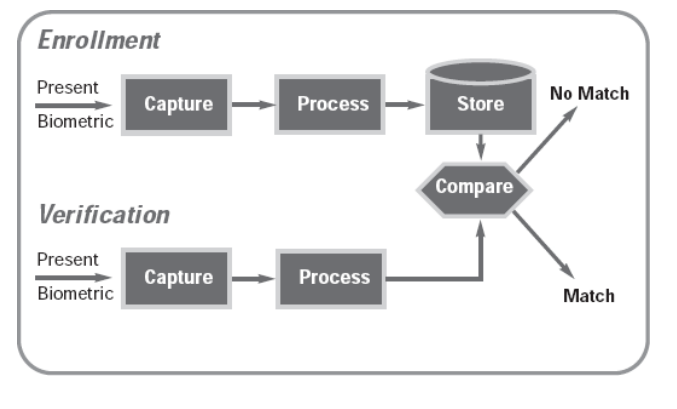
\includegraphics[scale=0.4]{screenshots/2026-11-08.png}
\end{center}
\begin{parag}{Verification}
    The second phase is Verification. Here the biometric is captured and processed as before, and the template obtained is compared to the stored one. Depending on which the following three phases happen we different security and privacy trade-offs: Capture: the sensor captures the biometric, Process: the captured biometric is converted on the template, Store: the template is stored
\begin{itemize}
    \item  Local: in the device where the assets that the biometrics protect are stored
    \item  Remote: on a server remote from the assets being protected
\end{itemize}

Storing/processing locally is more privacy-preserving, but harder to secure and difficult to update. Storing/processing remotely is less privacy-friendly (the server sees the biometrics),
but is easy to secure and update.
\end{parag}
\begin{parag}{What you are: Biometrics}
    As opposed to the hash in passwords, this comparison is not exact. Because the capture may contain differences (e.g. dirt of fingers, light when taking photos, etc), one has to decide a threshold to define what a match means.\\
	$ $\\
	When deciding this threshold one has to make a balance between false positives (how many times a biometrics that is not from the user is considered a match) and false negatives (how many times the user provides her biometrics, but these are rejected). What balance depends on the assets you are securing and what is more important, to keep them safe or to keep users happy.
\end{parag}

\subsection{Tokens}
\begin{parag}{Problems with Biometrics}
    \begin{subparag}{Hard to keep secret}
        Signature on ID card, fingerprint left on glasses, door handles, ..., photos! All of those require liveness detection: Liveness detection are measured in the capture/processing steps in which the users are required to do actions to demonstrate they are actually alive. 
    \end{subparag}
	\begin{subparag}{Revocation is difficult (impossible?)}
		Sorry, your irise has been compromised, please create a new one...
	\end{subparag}
	\begin{subparag}{Identifiable and unique}
	    Linking across systems
	\end{subparag}
	\begin{subparag}{May reveal private information}
	    
		\begin{itemize}
		    \item Iris $\to$ disease
		    \item Face $\to$ Identity
		\end{itemize}
		
	\end{subparag}

	\begin{subparag}{Not always universal or immutable}
	    Fingerprint disappear, iris changes with lenses, ...
	\end{subparag}
\end{parag}
After having see all of those issue let us try a new approach \important{tokens}. Recall from before that we also have authentication by proving ownership of a token. This proof can come by having a chip running a protocol on a secret. For instance, a smart card signs a challenge sent by the ATM to prove knowledge of a key.\\
$ $\\
Or from a device that contains a secret shared with the server. These device output a number based on this secret and time (require synchronization). The device is authenticated when it outputs the same number as the server.
\begin{parag}{Authentication}
    How it works could be the following 
	\begin{enumerate}
	    \item Step 1, Offline initialization: token and server establish a common \textit{seed} and synchronize their clocks
	    \item From then on, Operation: obtain a random number from the seed that can only be computed by the token
	\end{enumerate}
	The server asks to prove, the token computes which interval it is with respect to the time it was synchronized with the server.\\
	Then applies a keyed cryptographic function using as key the secret shared with the server n times on the seed, and sends the result to the server. Notice that from this value an adversary cannot recover the seed or the key (properties of encryption), and cannot compute future values because she does not have the key. The server does the same operation and checks
	
\end{parag}
\begin{center}
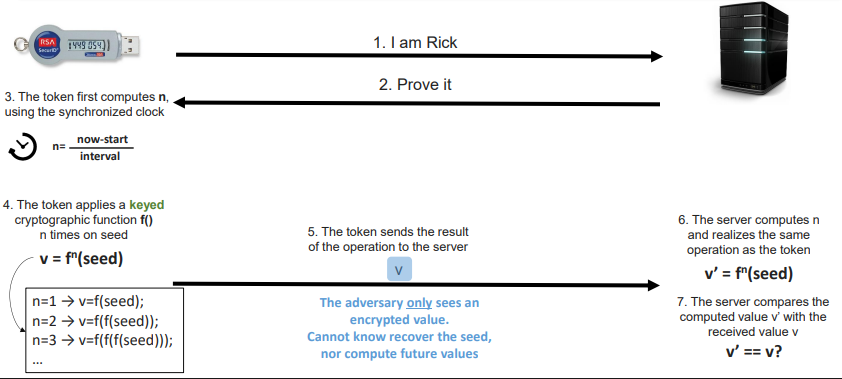
\includegraphics[scale=0.4]{screenshots/2026-11-08_1.png}
\end{center}
\begin{framedremark}
The reason we use a keyed function and not a hash is that everyone can compute a hash! If we use a hash instead of a keyed function, given $v$ I can produce any future $v$ by hashing the value!
\end{framedremark}


\begin{definition}{(2FA - Two factor authentication)}
	Combine two out of the three factors: (What you know, what you have, what you are)
\end{definition}

\paragraph{What machines have: Secret key}%
\label{par:What machines have: Secret key}
Finally, when we authenticate machine and not users, this is done using public key cryptography (e.g., to authenticate web servers). The authenticating party signs with their secret key. We use the secret keys to produce \important{digital signatures} to authenticate parties (e.g., used in the internet protocol HTTPS/TLS to authenticate the \important{server} (and can be used also to authenticate the client))
\begin{framedremark}
Building authentication protocols is \important{hard}
\begin{itemize}
    \item Defending from \important{man in the middle} --- Use signatures
    \item Defending from \important{replay attackscA --- uses challenges / nonces}
\end{itemize}
Even with that, it is still difficult to get right! One should use well established protocols (TLS 1.3, ISO 9798-3)
\end{framedremark}









